\section{Background: the foundational stochastic model of bedload transport} 
\label{sec:background}
 
\citet{Einstein1950} can be credited with the first attempt to understand the bedload flux as random quantity.  
Einstein understood the movement of individual bedload grains as a random succession of motion and rest intervals.
He termed the transition from rest to motion entrainment, and characterized it by a probability related to fluid turbulence. 
When particles are set in motion, Einstein considered they moved in discrete jumps of the same average distance. 
We define the bedload flux as the volume of grains passing a stream cross section per unit time.
It is a volume of grains per time per unit width of stream, so its units are $\text{area}/\text{time}$.  
Therefore, Einstein's mean flux formula is derived from summing the alternate start-stop motions of all bed particles which cross a surface in a time interval. 

The conceptual picture Einstein considered is depicted in figure \ref{fig:yalin}. 
All bed particles are identical and are considered to have the same average geometry when at rest on the bed, meaning their entrainment characteristics are identical. 
For continuity with the rest of the review, we consider sediment particles are spheres of radius $a$, although \citet{Einstein1950} was more general. 
We can follow Einstein to compute the mean number of these particles crossing a flow cross-sectional surface $S$ in an interval of time. 
This will construct the mean bedload flux $\bra q_s \ket$.
In subsequent sections, we consider $q_s$ a random variable, and we will review approaches to derive its full probability distribution.
From these contemporary models, an Einstein-like mean flux formula emerges from taking the mean of the probability distribution for $q_s$.  
Hence we use averaging brackets $\bra \cdot \ket$ for the sake of continuity. 
 
\begin{figure}
  \centering
  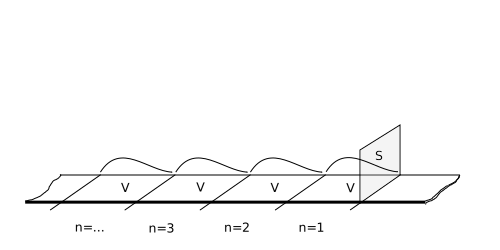
\includegraphics[width=.98\linewidth]{./figures/yalindrawing.png}
  \caption{Einstein's conceptual picture (adapted from \citet{Yalin1972}). Particles move in discrete jumps of length $L$ from left to right through an array of adjacent control volumes. The bedload flux is the volume of bedload particles crossing the surface $S$ per unit width and time. \label{fig:yalin}}
\end{figure}

Einstein's derivation goes as follows: we partition the channel into a sequence of identical control volumes $V$. 
Each volume has dimensions $L$, $w$, and $h$ ($V=lwh$). 
$L$ is the downstream length of each control volume, and it is also the average jump distance of particles. 
$w$ and $h$ are the width and height of each control volume.
Let $P_n$ be the probability that any individual grain on the bed is entrained \textit{at least} $n$ times during the time interval $T$. 
That is, let $P_n$ be the probability that an individual grain undergoes \textit{at least} $n$ jumps of length $L$ in an interval $T$, meaning it travels a distance $nL$ or more in $T$. 
Considering that each control volume contains $N_V$ grains at rest within it, it follows that on average
\be N_V P_n. \ee
grains are displaced \textit{at least} a distance $nL$ from a control volume within the time interval $T$.

Now we derive the mean flux. 
Note that the grains passing through a cross-sectional surface $S$ (of area $lw$) in the time $T$ could have come from any upstream location. 
Therefore, the number of grains crossing $S$ in $T$ is 
\be \sum_{n=1}^\infty N_V P_n. \ee
This is the net arrival of grains in the interval $T$ from all upstream control volumes. 
Multiplying by the particle volume $\nu_p$ and dividing by the timescale $T$ and channel width $w$ gives the mean bedload flux (volume per width per time):
\be \bra q_s \ket = \frac{\nu_p N_V}{w T}\sum_{n=1}^\infty P_n = A \frac{a^2}{T} \sum_{n=1}^\infty P_n. \label{eq:einstein1}\ee 
In the second equality, we have introduced $\nu_p = 4\pi a^3/3$, and two assumptions of Einstein. First, is the reasonable assumption that the number $N_V$ of particles on the surface within $V$ is proportional to the ratio of bed surface and particle areas: $N_V \propto Lw/a^2$, and second is the assumption that the travel distance $L$ is proportional to particle size: $L \propto a$. The latter assumption is more difficult to justify \citep[e.g.][]{Yalin1972}. 
$A$ is a constant of proportionality. 

Einstein implies the probability that an individual grain travels a distance $nL$ or more in $T$ is equivalent to the probability that an individual grain travels at least a distance $L$ successively $n$ times in $T$. 
Hence $P_n = P_1^n$ by the law of multiplication of probabilities, so that $\sum_{n=1}^\infty P_n = \sum_{n=1}^\infty P_1^n = P_1/(1-P_1)$, using the geometric series (noting $P_1 < 1$ because it is a probability). 
Owing to this substitution, Einstein's mean bedload formula takes the form 
\be  \bra q_s \ket = A \frac{a^2}{T}\frac{P_1}{1-P_1}, \label{eq:einstein2} \ee
where $A$ is a constant of proprotionality.  
The $P_1/(1-P_1)$ structure of Einstein's formula is a distinctive characteristic. 
In order to use the apply the Einstein formula to predict bedload transport in natural streams or experiments, the timescale $T$ and the probability $P_1$ that at least one grain entrains in $T$ must be determined. 
Then the formula can be calibrated to a given setting by adjusting the constant $A$.  

In the original work, Einstein considered the timescale $T$ proportional to the "time of the grain" formed by the grain's size $a$ and its settling velocity $w$ in still fluid: $T \propto a/w$. 
We will revisit this assumption shortly. 
Regarding the probability $P_1$, one of Einstein's most influential and enduring ideas within hydraulic engineering is his conception of the probability $P_1$ that at least one particle entrains in $T$. 
He considered that entrainment is driven by the fluctuating lift force imparted by the turbulent fluid, and it is resisted by the submerged weight of grains. 
Therefore, he formulated $P_1$ as an exceedance probability of the lift force over weight, so he wrote $P_1$ as an integral over the probability distribution of fluid shear stress. 
Einstein developed an alternative perspective on the incipient motion of particles that embraced turbulence and did not rely on the critical shear stress concept \citep[e.g.][]{Shields1936}.

This formulation of entrainment probability in terms of the exceedance of random driving quantities over (possibly random) resisting quantities has been generalized and extended a great deal. 
\citet{Paintal1971} made a significant extension by including random granular geometry of bed particles into the force balance. 
More recently, \citet{Tregnaghi2012} ammended the theory to include the impulse concept: the experimentally verified idea that force magnitude and duration are of equal importance for entrainment \citep[e.g.][]{Diplas2008, Celik2014}. 
Refined theories of the entrainment probability, all fundamentally similar to the original ideas of \citet{Einstein1950}, have been carefully reviewed by \citet{Dey2008, Dey2018}, and they are a subject of intensive ongoing research.  

As noted by \citet{Yalin1972}, who wrote a careful review and revision of \citet{Einstein1950}, the Einstein theory for $\bra q_s \ket$ is theoretically sound, at least to equation \ref{eq:einstein2}, and provided Einstein's probabilities $P_n$ are interpreted in a careful way. 
I have mimiced Yalin to say $P_n$ is the probability of \textit{at least} $n$ jumps in $T$. 
Had I said $P_n$ was the probability of (only) $n$ jumps in $T$, the relationship $P_n = P_1^n$ would not follow, so the Einstein flux would not develop the notable $P_1/(1-P_1)$ form as in \ref{eq:einstein2}. 
Einstein was not as clear as he could have been on this distinction. 
Notably, the more general birth-death theories which reproduce Einstein as a limiting case \citep[e.g.][]{Ancey2006} use probability concepts relating to (only) one entrainment in a time interval. 
Therefore, to link back to Einstein from these contemporary theories, we need to follow \citet{Yalin1972} to express the mean flux $\bra q_s \ket$ in terms of the probabilities of (only) $n$ entrainments in a time interval, which we can denote by a lower case letter $p_n$. 
These two probabilties, $P_n$ (at least) and $p_n$ (only), have probably been conflated often within the literature. 

Yalin appealed to scaling arguments in order to refine Einstein's theory. 
He highlighted that Einstein's prescription of $T \propto a/w$, where $w$ is the settling velocity, was not supported by any experimental evidence or theoretical argument. 
Yalin noted that within Einstein's theory, "$T$ appears in connection to the study of detachment of individual grains due to turbulent fluctuations", from which he concluded that $T$ should be actually be measured in terms of a period $\tau$ of turbulent fluctuations: 
\be T = N_\tau \tau, \label{eq:yalintime}\ee
where $N_\tau$ is the dimensionless number of turbulent fluctuations in $T$ (which is considered unknown but very large). 

Yalin introduces a probability $p$ of (only) one entrainment during an individual turbulent fluctuation. 
Since the number $N_\tau$ of turbulent fluctuations in $T$ is very large, he considers this probability is very small, so that the probability of (only) $n$ detachments in $T$ can be computed with the Poisson distribution: 
\be p_n = \frac{(N_\tau p)^n}{n!}e^{-N_\tau p}. \label{eq:yalinpoisson} \ee
The probability $P_n$ of \textit{at least} $n$ detachments in $T$ can be expressed in terms of the probability $p_n$ of (only) $n$ detachments in $T$ as 
\be P_n = \sum_{i=n}^\infty p_i. \label{eq:yalinsum}\ee
Owing to equations \ref{eq:yalintime}, \ref{eq:yalinpoisson}, and \ref{eq:yalinsum}, the mean bedload flux \ref{eq:einstein1} becomes
\be  \bra q_s \ket = A \frac{a^2}{N_\tau \tau} \sum_{n=1}^\infty \sum_{i=n}^\infty p_i = A \frac{a^2}{N_\tau \tau} \sum_{n=1}^\infty n p_n = A \frac{a L}{\tau} p. \label{eq:yalinflux} \ee
The unknown number of turbulent fluctuations $N_\tau$ cancels. 
Hence, Yalin's ammended Einstein formula is proportional to $p$, rather than $P_1/(1-P_1)$ as in \citet{Einstein1950}. 
In Yalin's mind, the probability $p$ is the probability of entrainment of only one grain in a small interval $\tau$ related to the period of turbulent fluctuations. 

When Einstein's conceptual picture of bedload transport is revisited from a Markov process framework, the probability distribution $P(q_s)$ of the bedload rate can be derived from his assumptions \citep{Ancey2006}. 
This distribution implies a mean bedload formula $\bra q_s \ket = \sum q_s P(q_s)$ formally similar to Yalin's Einstein-like formula \ref{eq:yalinflux}, and it provides additional information about the magnitude of bedload fluctuations, which are characterized without ambiguity by the variance $\bra \delta q_s^2 \ket$, where $\delta q_s = q_s - \bra q_s \ket$ is the deviation of the bedload flux from the mean.
Jumping ahead a little, the fluctuations $\bra (\delta q_s)^2 \ket$ derived in this way are not large enough to match experimental data \citep{Ancey2006}, and this is because \citet{Einstein1950}, \citet{Yalin1972}, and \citet{Ancey2006} each assumed the transitions between rest and motion were independent between all particles.
 
\citet{Ancey2008} fixed this problem by describing bedload transport within a more general birth-death process framework \citep{Cox1965}. 
They included a collective interaction into the entrainment rates of bed particles in their model, and with this inclusion they derived bedload fluctuations of realistic magnitude. 
Their collective interaction biases entrainment, making it more likely when particles are already moving, a point we will discuss.  
It leads to clouds of active particles, and a wide tail on the bedload flux probability distribution: both of these features are in accord with experimental observations \citep{Drake1988, Ancey2006, Ancey2008}. 
I'll start the review with \citet{Ancey2006}, which is essentially \citet{Einstein1950} revisited from the birth-death framework, lending it more generality by treating the bedload flux as a probability distribution.   
The mean of this probability distribution reproduces equation \ref{eq:yalinflux}, which is a satisfying historical coherence. 
Followups and refinements of the \citet{Ancey2006} work constitute the bulk of the review in section \ref{sec:review}. 

